% !TEX root = ../master-thesis.tex





\begin{figure}
    \centering
    \addletter{200}{a}
    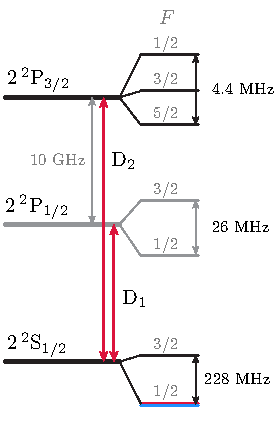
\includegraphics{fig-ai/li-levels-base.pdf}
    \hspace{1cm}
    \addletter{200}{b}
    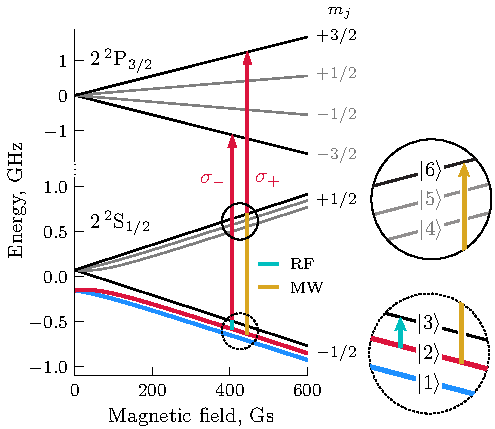
\includegraphics{fig-ai/li6-zeeman-broken-ai.pdf}
    \caption{
        \textbf{${}^6$Li energy levels}. 
        a) Level diagram of the ground and excited states of ${}^6$Li \cite{gehm_preparation_2003}, including the D1 and D2 transitions around $\lambda = 671$~nm. 
        b) Zeeman splitting of the hyperfine levels of the $2\, {}^2\mathrm{S}_{1/2}$ and $2\, {}^2\mathrm{P}_{2/2}$ in ${}^6$Li \cite{serwane_deterministic_2011, sibalic_arc_2017}. As different spin states for physics we consider state $\ket{1}$ and $\ket{2}$, but for imaging it is worth to flip them to stretched states $\ket{6}$, $\ket{3}$. Colored lines indicate transitions driven by radiofrequency (RF) and microwave (MW) fields.
    }
    \label{fig:li6levels}
\end{figure}


% \subsection{$^6$Li hyperfine structure and imaging scheme}

The $^6$Li atom possesses a relatively simple electronic structure that makes it well-suited for quantum gas experiments. The electronic ground state $2\,^2\mathrm{S}_{1/2}$ exhibits hyperfine splitting due to the interaction between the electron and nuclear spins, resulting in two manifolds with total angular momentum $F = 1/2$ and $F = 3/2$ separated by 228 MHz (Fig.~\ref{fig:li6levels}a). The excited $2\,^2\mathrm{P}$ states relevant for optical transitions around $\lambda = 671$ nm include both the $\mathrm{P}_{1/2}$ (D$_1$ line) and $\mathrm{P}_{3/2}$ (D$_2$ line) levels \cite{gehm_preparation_2003}.

For quantum simulation experiments, the two lowest hyperfine states $|F = 1/2, m_F = \pm 1/2\rangle$, commonly denoted as $|1\rangle$ and $|2\rangle$, serve as the effective spin-1/2 system for realizing the Fermi-Hubbard model. These states exhibit favorable scattering properties and can be brought into resonant interaction using Feshbach resonances near accessible magnetic field strengths.

However, for fluorescence imaging, the stretched states $|3\rangle$ and $|6\rangle$ offer significant advantages over the $|1\rangle$ and $|2\rangle$ states. As shown in Fig.~\ref{fig:li6levels}b, at magnetic fields above $\sim 100$ G, the stretched states acquire nearly pure $m_J = \pm 1/2$ character due to Zeeman splitting \cite{serwane_deterministic_2011, sibalic_arc_2017}. This results in strong coupling to circularly polarized light: state $|3\rangle$ couples primarily to $\sigma^-$ transitions while $|6\rangle$ couples to $\sigma^+$ transitions. The stretched nature ensures closed cycling transitions with minimal population leakage to other hyperfine states, enabling efficient photon scattering rates exceeding those achievable with $|1\rangle$ and $|2\rangle$.

The imaging protocol therefore involves a preliminary step where atoms are transferred from the $|1\rangle$ and $|2\rangle$ physics states to the $|3\rangle$ and $|6\rangle$ imaging states using radiofrequency or microwave pulses. The polarization selectivity of the stretched states then enables spatial separation of the fluorescence signals using polarizing optics, as detailed in Section 3.4. This approach preserves the spin information while optimizing detection efficiency through the enhanced scattering cross-sections of the stretched states.